\chapter{Squiggle alignment}

\label{kap:squiggles} % id kapitoly pre prikaz ref

In this chapter, we describe our work. 
We took a different approach from standard procedure described in \ref{standard}.
To compose DNA sequence, we took squiggles that correspond to the same part of the reference sequence and aligned them together to produce one signal that will be later basecalled. We designed several ways of multiple squiggles alignment to generate the best signal according to similarity of sequence from basecalling and reference sequence.

\section{Squiggles and preprocessing}

MinION device produces sequences of measured values of the current passing nanopores. We call these sequences squiggles.
Typically, we have multiple squiggles covering each part of the DNA. The raw signal contains values in pA between $0$ and several hundred. 
Each pore produces slightly different data. Current values are shifted and scaled by some constant.

The best way to hide these differences is to scale the sequence so that the resulting mean value is 0 and the standard deviation is one 
\cite{kubo}.

\section{Squiggle alignment with dynamic time warping}
To align two squiggles, we use the method called dynamic time warping (DTW).
DTW is widely used in audio processing and speech recognition \cite{muller2007dynamic}.
It uses a similar approach as the Needleman-Wunsch algorithm for sequence alignment, but 
does not specify the score of a match or a mismatch, but instead assigns a cost function for any pair of values.

The cost function $c(i,j)$ which assigns a cost for aligning value $i$ to value $j$. 
It can be, for example, distance $abs(i-j)$ or square of distance $abs(i-j)^2$.

By evaluating a cost function for two sequences $u$ and $v$, we calculate the cost matrix $C$, where $C[i,j] = c(u_i,v_j)$.
The best alignment of these two sequences can be represented as a continuous path from $C[1,1]$ to $C[n,m]$, with the lowest sum of costs (Fig. \ref{fig:wp}). 
We call such a path a warping path and the sum of costs will be the cost of the alignment. The cost of the alignment is also indicative of the similarity of those sequences.


\begin{figure}[h]
  \centering
  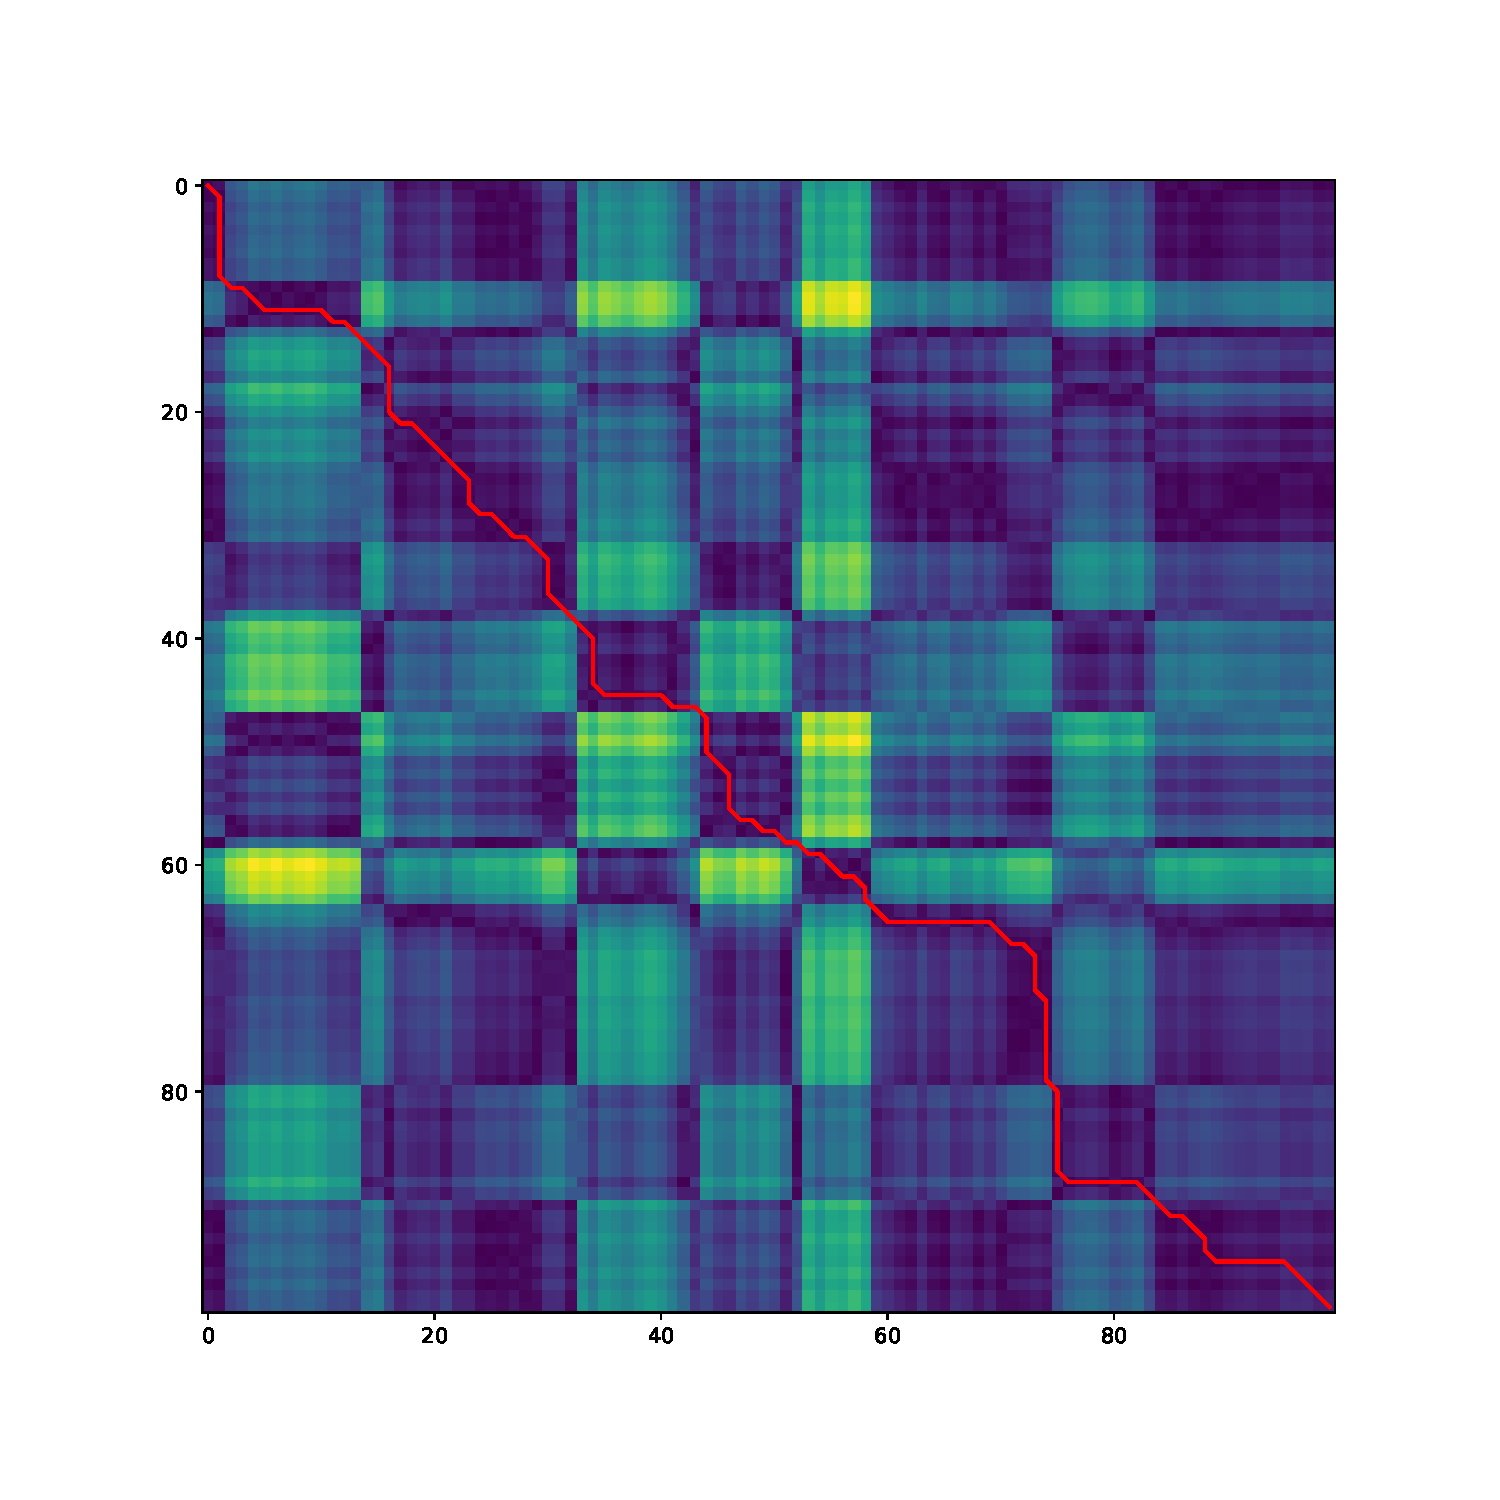
\includegraphics[width=0.8\textwidth]{images/wp}
  \caption{Warping path in matrix $C$.}
  \label{fig:wp}
\end{figure}

The warping path can be represented as a list of coordinates from matrix $C$.

To find the best path, we will not compute matrix $C$ containing the costs of aligning single values.
Instead, we will calculate matrix $A$, where $A[i,j]$ is the cost of the alignment of sequences $u_1 \dots u_i$ and $v_1 \dots v_j$, 
similarly as we did in the Needleman-Wunsh algorithm. 
In particular, $A[i,j]$ will be computed as $min(A[i-1,j],A[i,j-1],A[i-1,j-1])+c(u_i,v_j)$. 
To find the warping path in $A$, we follow the lowest values from $A[n,m]$ to $A[1,1]$. 

The time complexity of this algorithm is quadratic, but can be easily reduced to almost linear by restricting the area where the warping path is allowed to pass to a band with a constant width (Fig. \ref{fig:belt}). We will define $c(i,j)=\infty$ for all $i,j$ not in this band. This way, the values that are not computed, will not affect the final value. By checking the coordinates of a chosen point while constructing the warping path, we can find out if the chosen band covers the whole warping path. 
When the band is not wide enough, we will restart the computation with a band that will be twice as wide \cite{band}.
\begin{figure}[h]
  \centering
  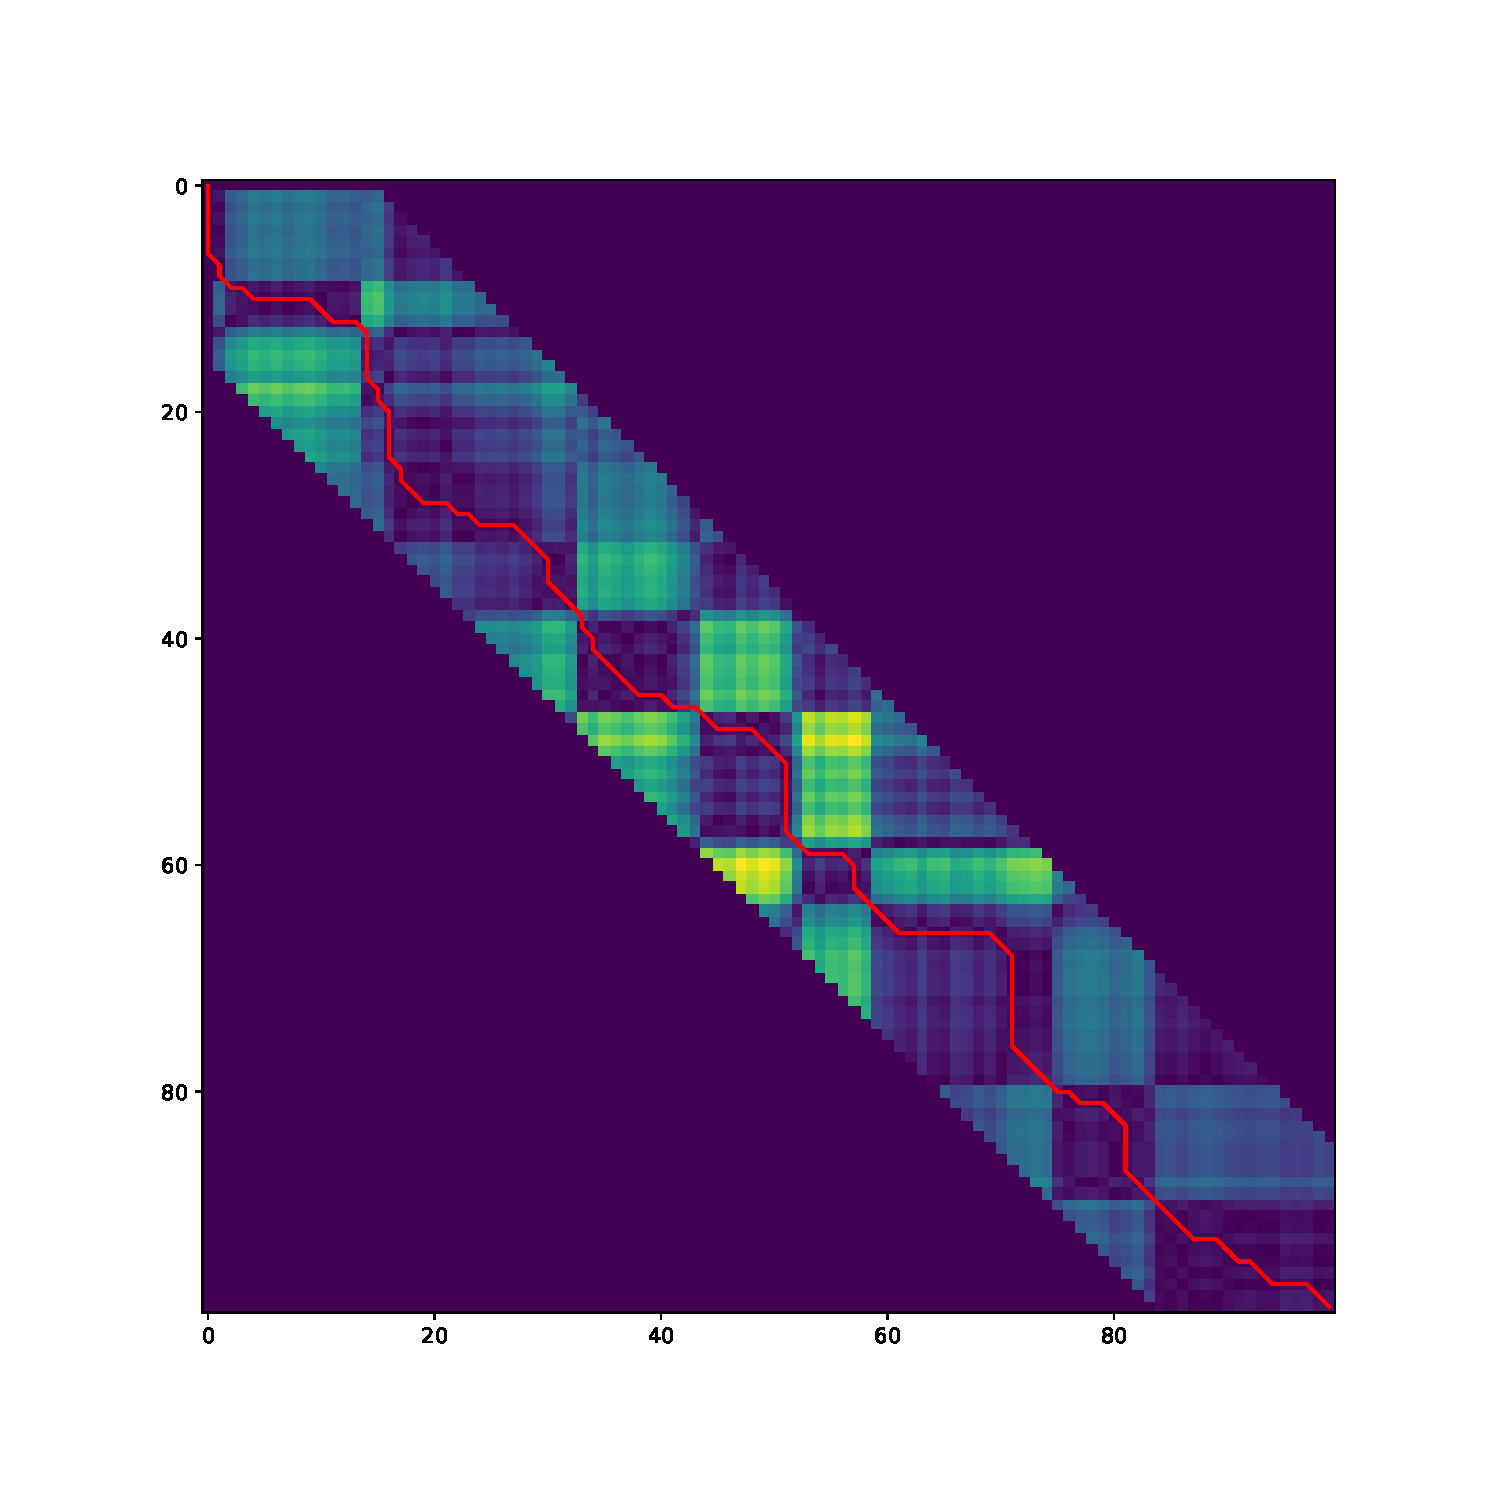
\includegraphics[width=0.8\textwidth]{images/wp2}
  \caption{Band restricted warping path in matrix $C$.}
  \label{fig:belt}
\end{figure}


\section{Signal reconstruction from the warping path}

To facilitate a progressive alignment of the squiggles, we need to be able to create one signal out of two. We will use the warping path created by DTW.
Although the signals are very similar, alignment still contains some insertions in both squiggles (Fig. \ref{fig:pairing}). 

\begin{figure}
  \centering
  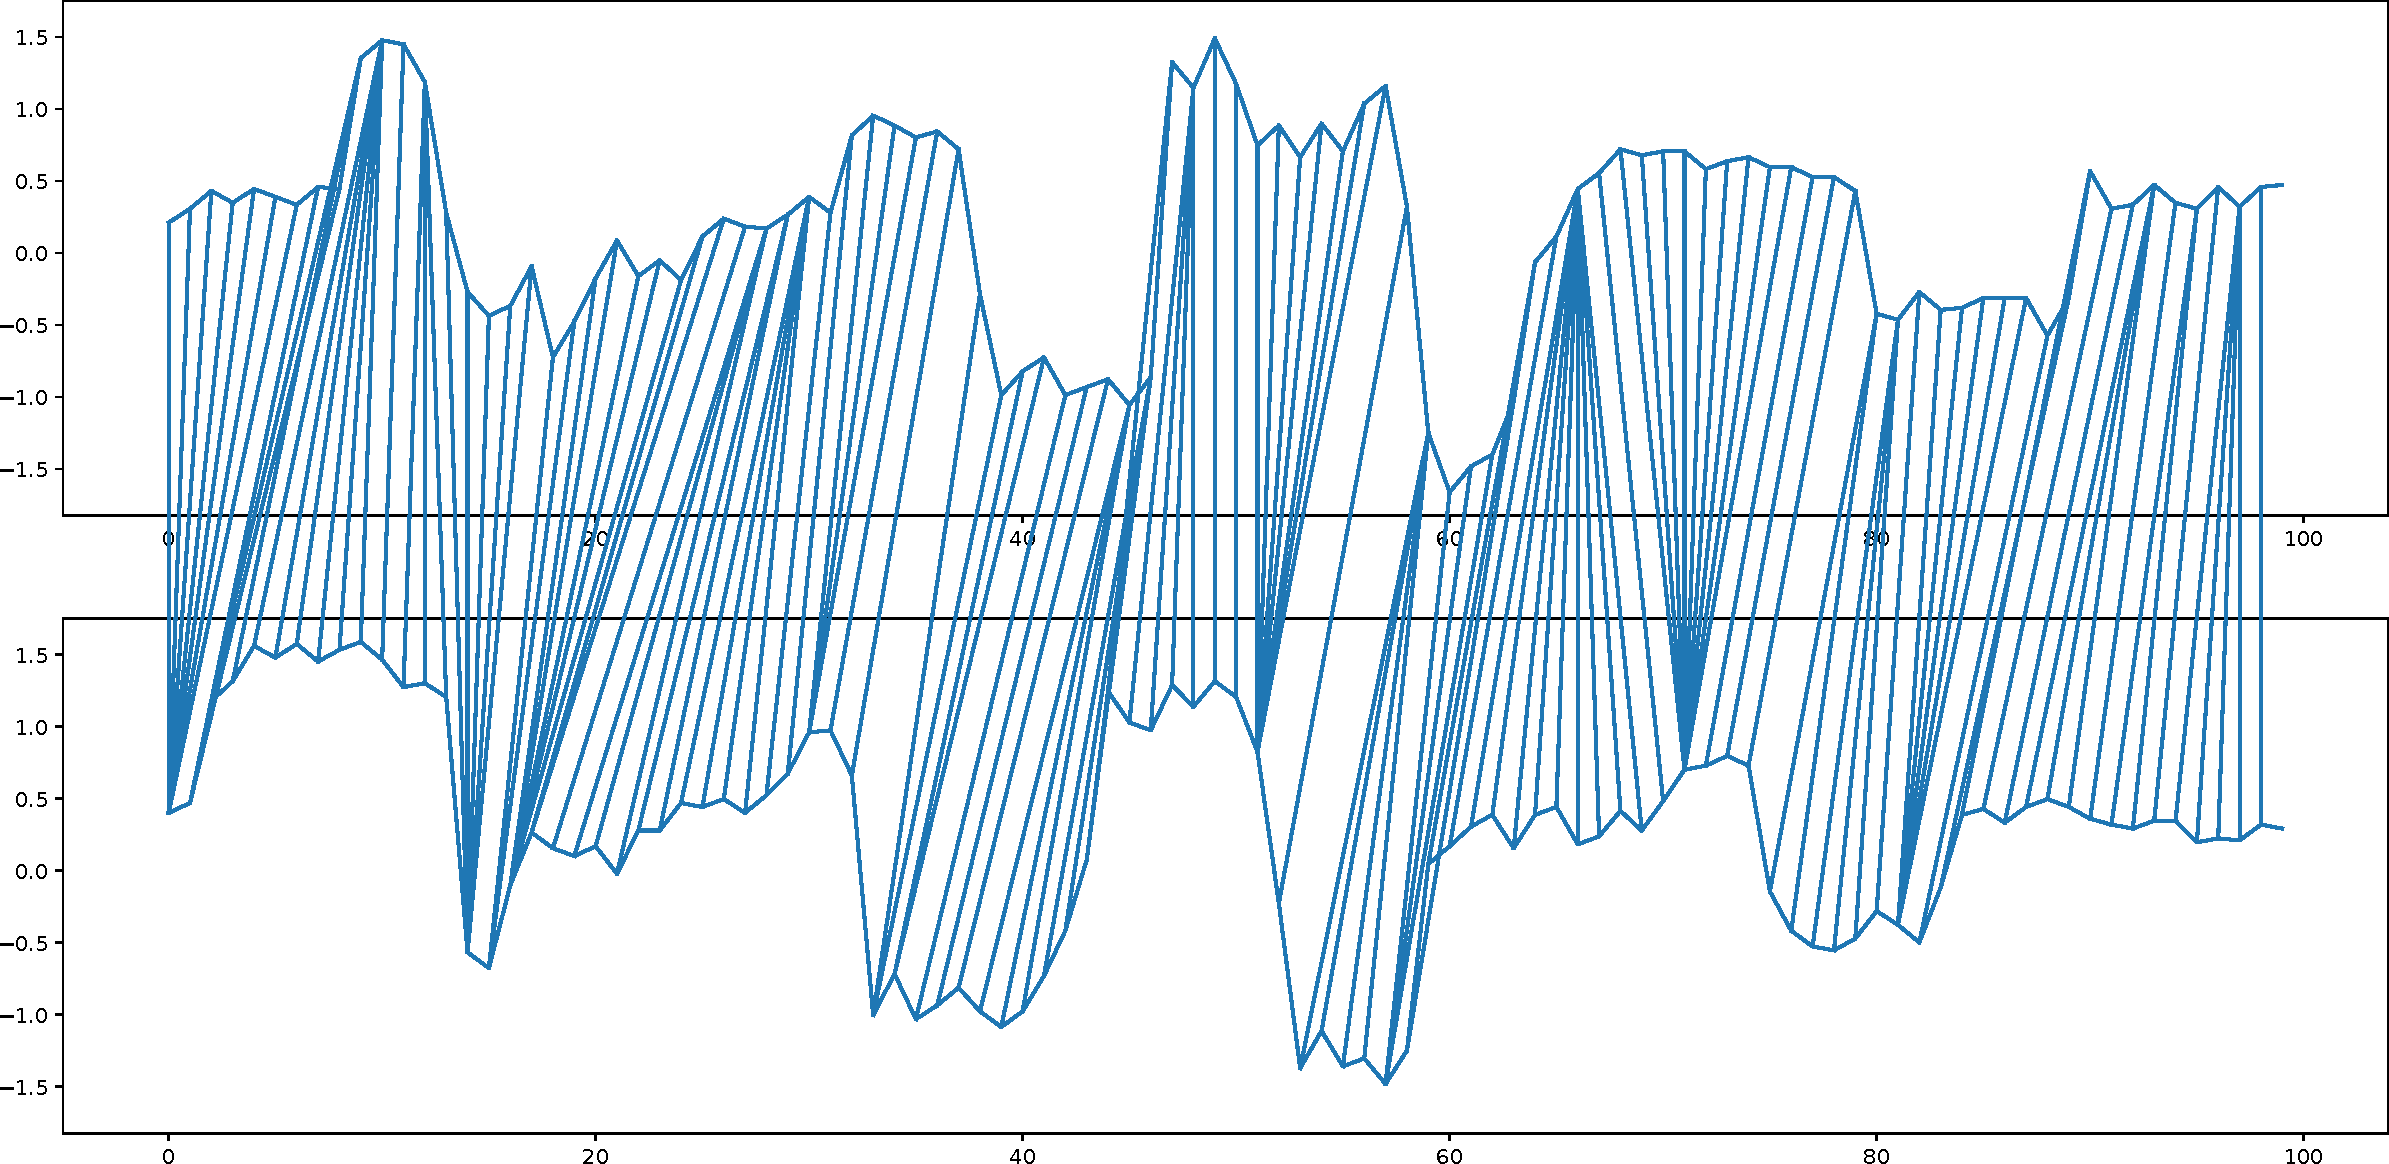
\includegraphics[width=1.0\textwidth]{images/ciary}
  \caption{Pairing of points created by DTW.}
  \label{fig:pairing}
\end{figure}

When aligning DNA sequences, we had three possibilities. Match, mismatch, or aligned to a dash. 
This time, we have a pairing of points. Each point from the first sequence has the corresponding point
in the second sequence and each point from the second sequence has the corresponding point
in the first sequence. This also means that sometimes one point from the first sequence corresponds to multiple points from the second sequence or vice versa.

We considered multiple ways to solve this problem.
\subsubsection{Complete alignment}
The first approach is to calculate an average of each pair of points in alignment and concatenate them to the final signal. The signal we create in this way is slightly longer.

\subsubsection{Alignment to sequence}
The second approach is to take the first sequence as leading and to construct the final signal by calculating an average of a point from this sequence and all points aligned to it, in every point of this sequence. 
This approach puts a high weight on the first sequence.
If some part of the signal from the second sequence is missing in the first sequence, it will never appear in the alignment.
The same holds if some parts of the first signal is unusually long. A single point from the second signal will align to it, and the whole length of the signal will stay there.
An advantage of this approach is, that the resulting signal looks exactly like a signal that MinION produces and the basecaller expect.

\section{Multiple alignment}

To align multiple signals, we have chosen the iterative method, as signals are much longer than the DNA sequences, and the iterative method is faster.
However if we would just add the sequences one-by-one and each time would generate a resulting signal, weight of the squiggles added later will be higher.
We have tried multiple approaches to solve this problem.
\subsubsection{Simple average}
The first approach was to calculate the weighted average when aligning the $i$-th signal to the consensus of $i-1$ already aligned signals. 
The result is that at each point, every sequence has the same weight in consensus.
\subsubsection{Average with length adjustment}
In the second approach, we remembered how many points were aligned from all sequences to each point of the consensus. We used
this information when reconstructing the final signal. For each point, we calculated an average number of points aligned to it and adjusted its weight in the final sequence accordingly.

With these different ways of reconstructing the final sequence, we can afford to take the full alignment each time. 
While it will result in much longer signal than expected, it will be later reduced by realigning all sequences to it and counting 
points aligned to each point in it.